\begin{pastexam}[label={px:ncu-114-dsa-06}]{中央資工所 114 學年度 第 6 題}
（複選；每題 5 分，全部答對才給分，答錯倒扣 1 分）

Consider a red-black tree with level order 50, 30, 80, 90. Which of the following statements is (are)
true?
\begin{enumerate}[label=(\alph*)]
\item node 30 is red.
\item After inserting 70 and 75, the level order traversal of the resulting red-black tree is 50, 30,
80, 70, 90, 75
\item After inserting 70 and 75, node 90 in the resulting red-black tree is black.
\item After inserting 70, 60, and 65, node 65 in the resulting red-black tree is black.
\end{enumerate}
\end{pastexam}

\begin{pastsoln}
答案：(b)(c)(d)。

\textbf{原來的樹和顏色}。 層序 50, 30, 80, 90 而且是二元搜尋樹，所以 $50$ 是根，$30$、$80$ 是它的
左、右子，$90$ 是 $80$ 的右子。 顏色由紅黑樹的性質決定（資結書第~10.3~節）：根 $50$ 是黑的。 從 $50$
往下到各個 \textsc{nil} 的路徑，黑節點數要一樣：
\begin{itemize}
\item 若 $80$ 是紅的，它的子 $90$ 必須是黑的；路徑 $50 \to 80 \to \textsc{nil}$（$80$ 的左邊）只有
$50$ 一個黑節點，$50 \to 80 \to 90 \to \textsc{nil}$ 有 $50$、$90$ 兩個，不相等。 所以 $80$ 是黑的。
\item $80$ 黑，路徑 $50 \to 80 \to \textsc{nil}$ 有兩個黑節點；$50 \to 30 \to \textsc{nil}$ 也要兩個，
$30$ 必須是黑的。
\item $50 \to 80 \to 90 \to \textsc{nil}$ 已經有 $50$、$80$ 兩個黑節點，$90$ 必須是紅的。
\end{itemize}
顏色唯一：$50$、$30$、$80$ 黑，$90$ 紅。 (a) 錯。

插入照資結書第~10.3.4~節：新節點先當紅色，依二元搜尋樹的規則放到葉子；父節點是紅的就要修正。
修正時看叔叔：叔叔紅就重新著色、問題往上移兩層；叔叔黑（含 \textsc{nil}）時，新節點、父、祖父
成一直線就在祖父做一次旋轉，成折線就先在父節點轉成一直線，再在祖父轉。

\textbf{插入 70、75}。
\begin{itemize}
\item $70$：$70 > 50$、$70 < 80$，放在 $80$ 的左邊，紅。 父 $80$ 是黑的，不用修正。
\item $75$：$75 > 50$、$75 < 80$、$75 > 70$，放在 $70$ 的右邊，紅。 父 $70$ 紅，叔叔 $90$ 也紅：
$70$、$90$ 改黑，祖父 $80$ 改紅。 $80$ 的父 $50$ 是黑的，結束。
\end{itemize}
\begin{center}
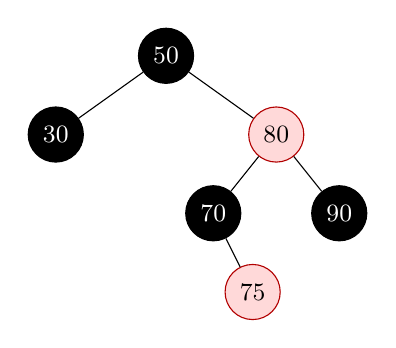
\begin{tikzpicture}[level distance=10mm,
  b/.style={circle,draw,fill=black,text=white,inner sep=1pt,minimum size=7mm,font=\small},
  r/.style={circle,draw=red!70!black,fill=red!15,inner sep=1pt,minimum size=7mm,font=\small},
  level 1/.style={sibling distance=28mm}, level 2/.style={sibling distance=16mm},
  level 3/.style={sibling distance=10mm}]
\node[b] {50}
  child {node[b] {30}}
  child {node[r] {80}
    child {node[b] {70} child[missing] child {node[r] {75}}}
    child {node[b] {90}}};
\end{tikzpicture}
\end{center}
（黑底白字是黑節點，淺紅底是紅節點。） 層序 50, 30, 80, 70, 90, 75，(b) 對；$90$ 是黑的，(c) 對。

\textbf{插入 70、60、65}（從原來的樹開始）。
\begin{itemize}
\item $70$：同上，放在 $80$ 的左邊，紅，不用修正。
\item $60$：$60 < 70$，放在 $70$ 的左邊，紅。 父 $70$ 紅、叔叔 $90$ 紅：$70$、$90$ 改黑，$80$ 改紅；
$80$ 的父 $50$ 黑，結束。
\item $65$：$65 < 70$、$65 > 60$，放在 $60$ 的右邊，紅。 父 $60$ 紅，叔叔是 $70$ 的右子 \textsc{nil}
（黑）。 $65$ 是右子、$60$ 是左子，成折線：先在 $60$ 左旋，$65$ 成為 $70$ 的左子、$60$ 成為 $65$ 的
左子；再在 $70$ 右旋，$65$ 升到 $70$ 原來的位置，改成黑色，$70$ 改成紅色。
\end{itemize}
\begin{center}
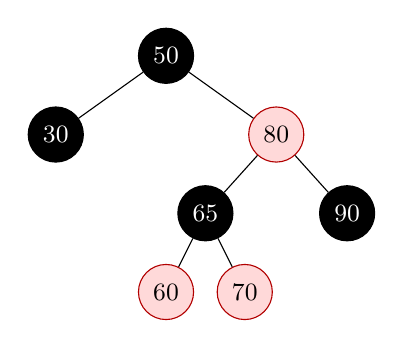
\begin{tikzpicture}[level distance=10mm,
  b/.style={circle,draw,fill=black,text=white,inner sep=1pt,minimum size=7mm,font=\small},
  r/.style={circle,draw=red!70!black,fill=red!15,inner sep=1pt,minimum size=7mm,font=\small},
  level 1/.style={sibling distance=28mm}, level 2/.style={sibling distance=18mm},
  level 3/.style={sibling distance=10mm}]
\node[b] {50}
  child {node[b] {30}}
  child {node[r] {80}
    child {node[b] {65} child {node[r] {60}} child {node[r] {70}}}
    child {node[b] {90}}};
\end{tikzpicture}
\end{center}
$65$ 是黑的，(d) 對。 檢查：每條根到 \textsc{nil} 的路徑都有 $3$ 個黑節點（例如 $50, 80, 65, 60$
之下的 \textsc{nil}：黑的是 $50$、$65$ 和 \textsc{nil}），沒有紅節點有紅子。
\end{pastsoln}
